%%%%%%%%%%%%%%%%%%%%%%%%%%%%%%%%%%%%%%%%%%%%%%%%%%%%%%%%%%%%
%%
%% LaTeX Thesis Template defined by Anthony Faustine(sambaiga@gmail.com), 2016
%%
%%%%%%%%%%%%%%%%%%%%%%%%%%%%%%%%%%%%%%%%%%%%%%%%%%%%%%

\RequirePackage[l2tabu, orthodox]{nag}  %checks for obsolete LaTeX packages and outdated commands


\documentclass[a4paper,12pt]{article}
 
\usepackage{setspace} %set line spacing
\doublespacing
% or:
%\onehalfspacing
\setlength{\parindent}{0pt} %set noindent for all paragraphs
\setlength{\parskip}{2.0ex plus0.5ex minus0.2ex}


% package imports
\usepackage{amsmath,amsthm,amssymb,amsfonts} %for math environments

\usepackage{a4wide}  % Pulls the page out a bit - makes it look better (in my opinion)
\usepackage{parskip}  % Removes paragraph indentation (not needed most of the time now)
\usepackage{fullpage}
\usepackage{blindtext}
\usepackage{algorithm}
\usepackage[pdftex]{graphicx}
\usepackage{float}
\usepackage{subfig}
\usepackage{siunitx}  % for writing scientific documents, where units and numbers are a big part of the writing.
\usepackage{booktabs} % To create tables without vertical separators.
\usepackage[table,xcdraw]{xcolor}
\usepackage{multirow} %for table with multi column
\usepackage{color}
\usepackage{algorithm}
\usepackage{algorithmic} %for algorithm
\usepackage[round]{natbib} %for citation 
\usepackage[margin=10pt,font=small,labelfont=bf, labelsep=endash]{caption}% Vastly improves the standard formatting of captions
\usepackage{todonotes}
\usepackage[margin=1in]{geometry}
\usepackage{bm}
%\usepackage{apacite}
%\usepackage{subfigure} % Provides commands to make subfigures (figures with (a), (b) and (c))
\usepackage{pdflscape} %for land scapping pages
\usepackage[final]{microtype} %improves the spacing between words and letters
\usepackage{footnote}
\usepackage[hidelinks]{hyperref}
%\usepackage{pslatex}
\usepackage{times}
\usepackage{lipsum}  %Generate dummy text (lorem ipsum) in your document


% settings
%\bibliographystyle{plain}
\setcounter{secnumdepth}{3}
\setcounter{tocdepth}{3}
\pagenumbering{roman}



\setlength{\textheight}{9.8in} \setlength{\topmargin}{0.0in}
\setlength{\headheight}{0.0in} \setlength{\headsep}{0.0in}
\setlength{\leftmargin}{0.0in}
\setlength{\oddsidemargin}{0.0in}
%\setlength{\parindent}{1pc}
\setlength{\textwidth}{6.5in}
%\linespread{1.6}

% Useful custom commands
\newcommand{\note}[1]{\color{blue}#1\color{black}}
\newcommand{\missref}{\note{[REF]}}


\newcommand{\etal}{\textit{et.~al.}}
\newcommand{\phys}{\textit{Physarum Polycephalum}}

% The document starts here



  
\begin{document}

\newcounter{rom}
 
\begin{titlepage}
     \centering
        \vspace*{0.5cm}
        
       {\Large \textbf{Nelson Mandela African Institution of Science and Technology(NM-AIST)}} \\[1.5 cm]
        
        
\includegraphics[width=0.4\textwidth]{images/logo} \\[1.5 cm]
        
        {\large \textbf {School of Computational Science and Communication Engineering}} \\[0.5 cm]
        
       {\large \textbf {PhD Research Proposal}} \\[1.0 cm]
       
   {\Large \textbf{Non-Intrusive Load Monitoring Framework for Sustainable Energy Consumption in Residential  Buildings} } \\[1.0 cm]

	

   { \normalsize \textbf{Student: Anthony Faustine (Reg.No:P158/T.15) }} \\[0.5cm]
            {\normalsize \textbf{ B.Sc (ESC., UDSM) and M.Sc.(Telecom Eng., UDOM) }} \\[0.5cm]
 
 \begin{tabular}{l l}
  {\normalsize \textbf{Supervisors:} } &{\normalsize \textbf{Prof.Nerey Mvungi,}} \\
   &{\normalsize \textbf{Dr. Kisangiri Michael,}} \\
   &{\normalsize \textbf{Dr. Shubi Kaijage.}}

\end{tabular}


   
							 
    \vfill
    
\end{titlepage}
 \cleardoublepage
 \begin{center}
 	%	\thispagestyle{empty}
 	\vspace*{.15\textheight}
 	
 	

 	
 	Approved by: 
 	\bigbreak
 	
 	\noindent\begin{tabular}{ll}
 		\makebox[2.5in]{\hrulefill} & \makebox[2.5in]{\hrulefill}\\
 		Dr.Kisangiri Michael & Date\\[8ex]% adds space between the two sets of signatures
 		\makebox[2.5in]{\hrulefill} & \makebox[2.5in]{\hrulefill}\\
 	Dr. Shubi Kaijage & Date\\
 	\end{tabular}
 	
 	
 
 \end{center}
 
\addtocounter{rom}{1}\setcounter{page}{2}~
\newpage\thispagestyle{plain}\setcounter{page}{3}
 
\tableofcontents
\listoffigures
\listoftables
%\newpage\thispagestyle{plain}~
\clearpage
\pagenumbering{arabic}

\section{Introduction}
Worldwide electrical energy consumption is constantly increasing especially in developing countries \citep{Monacchi2013}. According to United States Energy Information Administration report\footnote{http://www.eia.gov/todayinenergy/detail.cfm?id=14011}, \textit{the developing countries will account for 65\% of the global energy consumption by 2040}. 

\lipsum[1]

\subsection{Background}

Over the recently most part of the world has witnessed rapidly increasing to energy use in buildings (residential and commercial). Building contribute about 40\% of the total global energy \citep{Batra2014c}. Residential and commercial buildings consume approximately 60\% of the world’s electricity \footnote{The United Nation’s Environment Programme’s Sustainable Building and Climate Initiative (UNEP-SBCI)}. In U.S. A for example 74.9\% of all the electricity produced is used just to operate buildings \footnote{\href{http://www.eia.gov/todayinenergy/detail.cfm?id=14011}{United States Energy Information Administration report}} while in Africa, 56\% of the total electric power demand is from buildings \citep{Kitio2013}. Thus, energy saving in buildings will have significant impact on the reduction of overall energy consumption.

\lipsum[1]

\subsection{Problem Statement}

The key challenge to NILM problem is how to design efficient unsupervised NILM algorithm that can run in real-time using low-frequency sampling data. Several state-of-the-art NILM algorithms have been proposed using different approaches such as different variants of Hidden Markov Models (HMM) \citep{Kim2011,Parson2012,Kolter2012,Makonin2015}, Deep Neural Networks (DNN) \citep{Badayos2015,Paulo2016a}, Graph Signal Processing (GSP) \citep{Stankovic2014,Zhao2016a} and Combinatorial Optimization (CO) \citep{ReyesLua2015,Batra2013}. However, most of these algorithms suffer from high computational complexity which make them unstable for real-time applications, cannot be generalized across different buildings, requires lot of training data, their performance is limited to few numbers of appliances and are sensitive to noise and similar devices

\lipsum[1]
\subsection{Research Objectives}

\subsubsection{Main Objective}

The broad aim of this study is to develop NILM framework for sustainable residential buildings energy. The NILM framework will be well suited for the inherent characteristics of grids in Tanzania.

\subsubsection{Specific Objectives}
Specific Objectives are:
\begin{enumerate}
	\item To develop tools that will enable disaggregation research in developing countries.
	\item To develop innovative and real-time unsupervised NILM algorithms for sustainable energy consumption in residential buildings.
	\item To demonstrate and evaluate the potential of the proposed algorithm in (2) for sustainable
	energy consumption in residential buildings .
\end{enumerate}

\subsection{Research Questions}
This research is intended to answer the following questions:
\begin{enumerate}
	\item What tools can be developed to increase energy disaggregation research in developing countries?.
	\item How to design an efficient and real-time NILM algorithms that can be generalized across buildings  by taking into consideration developing countries characteristics?.
	\item Which and how innovative sustainable energy saving applications in residential buildings could be enabled with NILM algorithms in (2)?.
\end{enumerate}

\subsection{Significance of the Research}
The major contribution of the proposed study will be  novel unsupervised algorithm for energy disaggregation problem and its applicability in helping households to achieve quantifiable energy saving. The algorithm will provide real-time appliance specific information that will increase public awareness and make them be part and parcel of energy conservation. It will further help utility and policy makers gain better insights into energy consumption in residential buildings. 

The proposed study will establish tools and resource pertaining to energy consumption data sets. This will facilitate and promote research activities in energy disaggregation, energy data analysis, electricity grid modelling and appliance usage behaviour. Apart from that, energy consumption data sets  will be useful for policy makers in the energy sector.

The study will also contribute to the  understanding of challenges and possible strategies for energy conservation in residential buildings. Finally, the proposed study is expected to provide better theoretical understanding of NILM and its applicability in sustainable energy in residential buildings. 
\section{Literature Review}

\lipsum[2]

\subsection{Non-Intrusive Load Monitoring}

Non-Intrusive Load Monitoring (NILM) also known as energy disaggregation, is a computational techniques that estimates the energy consumed by every individual appliance given just a whole-house power measurements acquired from a single point source such as smart meter. This technique is gaining popularity due to large-scale smart meter deployments worldwide \citep{ReyesLua2015}. 

The big challenge to NILM problem is how to design  algorithm that can accurately perform energy disaggregation. Specifically, the problem of energy disaggregation can be formulated as follows: Given the sequence of aggregate power consumption $\bm{X} = \{X_1,X_2...,X_T \}$ from $N$ active appliances at the entry point of the meter at $\bm{t}=\{1, 2..., T\}$. The task of the NILM algorithm is to infer the power contribution of each of the $N$ appliances, that is,
\begin{gather*}
Y^{(1)} = \{y_1^1, ...,y_T^1\}\\
Y^{(2)} = \{y_1^2, ...,y_T^2\}\\
\vdots \\
Y^{(N)} = \{y_1^N, ..., y_T^N\}
\end{gather*} as shown in Figure \ref{fig:NILM}, such that at any point in time $t$, $$X_t = \sum_{i=1}^N y_t^i + \sigma(t)$$, where $y_t^i$ is the power load of appliance $i$ at time $t$ and $\sigma(t)$ represents both any contribution from appliances not accounted for and measurement noise.
\begin{figure}[ht]
	\centering
	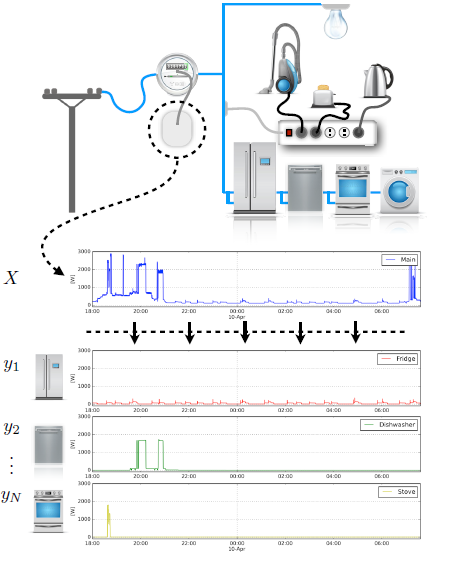
\includegraphics[width=0.5\textwidth]{images/NILM.pdf}
	\caption[An illustration of Non Intrusive Load Monitoring (NILM)]{An illustration of Non Intrusive Load Monitoring (NILM).The goal is to retrieve the individual
		appliance signals $(yi)$ from the total power consumption $X_t$ \citep{Huss2015}}
	\label{fig:NILM}
\end{figure}

A typical NILM algorithm consists of the following steps: power signal acquisition, event detection, feature extraction and inference and learning.

\subsubsection{Power Signal Acquisition}

\lipsum[2]

High-frequency sampling is the measurement of electrical characteristics sampled at a much higher frequency in a range of \SIrange{10}{100}{\mega\hertz}. Power meters at this sampling rates are often custom-built and expensive due to sophisticated hardware \citep{Zoha2012}.

On the other hand, low-frequency sampling is the measurements of the power signal at a rate less than \SI{1}{\hertz}. Smart meters belong to this category since it communicate readings every \SIrange{1}{5}{\second} (\SIrange{0.2}{1}{\hertz}). This research specifically, focus on low-frequency sampling since power data at this sampling can be obtained from smart meters which are being deployed in increasing numbers by utilities worldwide.

\subsubsection{Event Detection}
\lipsum[1]

\textbf{Event-Based Approaches:} The event-based approaches focus on the ON/OFF edges generated by appliances and use change detection algorithm to identify start and end of an event \citep{Barsim2014,Wong2013}.

\lipsum[1]
\begin{figure}[ht]
	\centering
	\includegraphics[width=0.5\textwidth]{images/edge.pdf}
	\caption[Edge-based schematic ]{Schematic of Edge-based \citep{ZhaoyiKang2015}}
	\label{fig:edge}
\end{figure}

\textbf{State-based Approaches:} State-based  State-based NILMs are usually based in HMM and its variants \citep{Kim2011,Kolter2012,Parson2012,Makonin2015} .
\lipsum[2]


\subsection{State-of-the-arts NILM Algorithms}


Several state-of-the-art NILM unsupervised algorithms have been proposed using different approaches such as different variants of Hidden Markov Models (HMM), Graph Signal Processing (GSP) and Deep Neural Networks (DNN). 

\subsubsection{Hidden Markov Model}
HMM is a Markov model whose states are not directly observed instead each state is characterised by a probability distribution function modelling the observation corresponding to that state \citep{Kim2011,Rabiner1989a}. There are two variables in HMM: observed variables and hidden variables where the sequences of hidden variables forms a Markov process. In the context of NILM, the hidden variables are used to model states(ON,OFF, standby etc) of individual appliances and the observed variables are used to model the electric usage. HMMs has been widely used in most of the recently proposed NILM approach because it represents well the individual appliance internal states which are not directly observed in the targeted energy consumption.

A typical HMM is characterised by the following: The finite set of hidden states $S$ (e.g ON, stand-by, OFF, etc.) of an appliance, $S = \{S_1, S_2....,S_N\}$. The finite set of observable symbol $Y$ per states (power consumption) observed in each state, $Y = \{Y_1, Y_2....,Y_M\}$. The observable symbol $Y$ can be discrete or a continuous set. The transition matrix \textbf{A} $=\{a_{ij},1\leq i,j \geq N\} $ represents the probability of moving from state $S_i$ to $S_j$ such that:
$a_{ij} = P(q_{t+1} =S_j \mid q_t=S_i)$, with $a_{ij} \leq 0$ and where $q_t$ denotes the state occupied by the system at time $t$. The emission matrix \textbf{B}$ =\{b(O \mid S_j)\} $ representing the probability of emission of symbol $O$ $\epsilon$ $ Y$ when system state is $S_j$. And the initial state probability distribution $\bm{\pi} = \{\pi_i \}$ indicating the probability of each state of the hidden variable  at $t = 1$ such that, $\pi _i = P(q_1 = s_i), 1 \leq i \geq N$. 

The set of all HMM model parameters is represented by 
$\bm{\lambda =\{\pi, A, B \}}$.~Several HMMs based NILM algorithms for energy disaggregation at low sampling rate has been proposed in the literature.


\cite{Kim2011} propose  an unsupervised technique for energy disaggregation using a combination of four FHMM variants. They use low-frequency real power feature and assume a binary state of appliances. To learn model parameters, Kim's approach uses Expectation Maximasation(EM) algorithm  and employ Maximum Likelihood Estimation(MLE) algorithm to infer load states. The performance of Kim's technique quickly decreases as the number of appliances increases and can only identify up to 10 appliances \citep{Parson2014c}. In addition, the reported work require appliances to be manually labelled after disaggregation and suffer from high computational complexity which makes it unstable for real-time applications.



\subsection{Energy Datasets}
\lipsum[1] 

Recent years has seen the emergency of several publicly available datasets such as UK-DALE \citep{Kelly2015}, AMPDs and AMPDs2 \citep{Makonin2013,Makonin2016}, ECO dataset \citep{Beckel2014}, REFIT dataset \citep{Murray2015b} and GREED dataset \citep{Monacchi2015a}. The comparison of various publicly available dataset with their characteristics is shown in Table \ref{tab:dataset}. This comparison is an extension of the proposed one in \citep{Bonfigli2015} and \citep{Murray2015b} with an update of the recent published data and additional data on included in some datasets. However, most of the datasets are from USA and some from European countries besides Canada and India. To the knowledge of researcher, there is no open-access dataset recorded in Tanzania. According to \cite{Kelly2015} to test the performance of a NILM algorithm for a specific country, it is important to have access to data from that country. This is because electricity usage varies significantly between countries owing to different use of sets of appliances and different cultures. Using dataset recorded from different countries could lead to mismatching of electric quantities. For example, while most of existing datasets recorded from USA where the RMS voltage value is \SI{120}{\volt}, most of developing countries including Tanzania work under \SI{240}{\volt} RMS voltage. The study will develop energy data set containing detailed power usage information obtained from well-instrumented residential buildings in Tanzania. Availability of these data set will promote research activities in energy consumption, data analysis and provide understanding of Tanzania domestic power usage and consumption.

\begin{landscape}
	\begin{table}[]
		\centering
		\caption{Publically Available Energy Dataset Comparison}
		\scalebox{0.75}{
			\begin{tabular}{p{4cm}p{2cm}p{3cm}p{2cm}p{3cm}p{5cm}p{5cm}p{7cm}}
				\toprule
				Dataset & Location & Duration & Number of houses & Sensors per house & Sample resolution & Features & Other Data \\
				\midrule
				REDD \citep{Kolter2011} & USA & 3-19 days & 6 & 24 & 15KHz(Aggr), 0.5Hz and 1Hz (sub) & V and P (Aggr), P (sub) &  \\
				BERDS \citep{Maasoumy2013} & USA & 1 year & 1 & 4 & 20sec & P,Q and S & climate data \\
				BLUED \citep{Anderson2012a} & USA & 8 days & 1 & Aggregated & 12KHz(Aggr only) & I, V and State transition label for each appliance. &  \\
				Smart \citep{Barker2012a} & USA & 3 months & 3 & 21-26 circuit meters & 1Hz & P and S (Aggr), P (Sub) & electricity generation data from on-site solar panels and wind turbines, outdoor weather data, temperature and humidity data in indoor rooms \\
				Tracebase \citep{Reinhardt2012} & Germany & N/A & 15 & 158 devices & 1-10sec(Sub only) & P &  \\
				AMPDS \citep{Makonin2013} & Canada & 1 year & 1 & 19 & 1min & V, I, F P, Q, S and Pf & water and natural gas, \\
				AMPds2 \citep{Makonin2016} & Canada & 2 & 1 & 21 & 1min & V, I, F P, Q, S , Pf ,real energy, reactive energy, and apparent energy & water and natural gas, weather data and   utility billing data. \\
				UK-DALE \citep{Kelly2015} & UK & 499 days, 2.5 years(house 1) & 5 & 5-54 devices & 16 kHz(Aggr) and 1/6 Hz(Sub) & P and switch status &  \\
				iAWE \citep{Batra2013} & India & 73 days & 10 & 33 devices & 1sec(Aggr) and 1sec or 6sec (Sub) & V, I, F, P and phase & Water and ambient conditions \\
				REFIT \citep{Murray2015} & UK & 2years & 20 & 11 & 8sec & P & Gas and environmental data \\
				GREED \citep{Monacchi2015a} & Australia/Italy & 1year & 9 & 9 & 1Hz & P &  \\
				ECO \citep{Beckel2014} & Switzerland & 8months & 6 &  & 1Hz & P and Q & Occupancy information \\
				IHEPCDS \footnote{http://archive.ics.uci.edu/ml/datasets/Individual+household+electric+power+consumption} & France & 4 years & 1 & 3 & 1min & V, I, P and Q &  \\
				OCTES \footnote{http://octes.oamk.fi/final/} & Scotland,Iceland \&Finland & 4–13months & 33 & Aggregated & 7sec & P and phase &  \\
				HES & UK & 1month(255 houses), 1year(26houses) & 251 & 13-51 & 2min & P &  \\
				ACS-F1 \citep{Gisler2013} & Switzerland & 2, 1 hoursessions & NA & 100, 10 types & 10sec & P, Q, I, f, V and phase & \\
				\bottomrule 
			\end{tabular}%
		}
		\label{tab:dataset}%
		\raggedright{\textit{Aggregte (Aggr), Sub-metering (sub), Active Power (P), Reactive Power (Q), Apparent Power (S), Energy (E), Frequency (f), Voltage (V) and Current (I)}}
	\end{table}
\end{landscape}
\subsection{Conclusion}
Despite the major leaps forward in the field, the electricity disaggregation problem is by no means solved; no convincing results have been presented for a precise and reliable method that is general enough to be deploy in any household.























































































































































































































































































































































































































































































































































































































































































































\section{Research Methodology}
To achieve the research aim along with its objectives, this research will be grounded in design science research. Design science research is a problem-solving based research methodology that is focused on creation and investigation of technological artifacts  \citep{Hevner2004,Dresch2015,Wieringa2014}. It is oriented in solving a specific problems with the aim to obtain a solution that is liable to generalization for a specific class of problem even if the solution is not optimal \citep{Dresch2015}.

Since the main objective of this study is to develop NILM framework for sustainable energy in residential buildings, design science research gives the necessary framework for implementation of the proposed study. Through an iterative Vaishnavi and Kuechler's design cycle \citep{Tobergte2013}, the research will first create innovative artefacts which aims to improve energy efficiency in residential buildings and evaluate these concepts by providing concretes 
instantiation. 
\begin{figure}[ht]
	\centering
	\includegraphics[scale=0.48]{images/DSP1.pdf}
	\caption{Research Design}
	\label{fig:design_science}
\end{figure}

The research design is divided into five phases summarized in Figure \ref{fig:design_science}:

\textbf{Theory building:} The first phase of this study will be focused on literature review in the domain of NILM and its applicability in energy conservation in residential buildings. The purpose of literature review  to summarize the existing research and provide
future guidelines for research by identifying gaps in the existing literature \citep{Compton1993}. It allows the desired information to be extracted from an increasing volume of published results \citep{Seuring2012}. This will help to provide better understanding of the NILM problem, build a theoretical and practical framework related to a specific research questions and demarcate the scope of the study. For this study literature review will always be used as first step of knowledge acquisition.


\textbf{Empirical research:} In the second phase, building-block approach and experimental research will be used. The building-block approach will be employed in the development of a system that will facilitate collection of energy-data set in residential buildings. Building-block approach is a design method  for designing systems in which independently prepared modules are combined to form the final products \citep{Dutta2008}. The approach is suitable for this study as it allows for rapid prototyping and "try it and see" experimentation. 

The developed tools will be instrumented in one residential home in Tanzania  for one year. This will be used to gather ground truth electricity usage data from wide variety of loads as well the whole-house consumption at low sampling rate. The output of this experiment will lead to the establishment of the first energy datasets from Tanzania. The developed energy datasets will be technically validated using the Non-Intrusive Load Monitoring Toolkit (NILMTK)\footnote{http://nilmtk.github.io/} NILMTK. NILMTK is an open-source NILM toolkit written in Python and designed specifically to enable the comparison of NILM algorithms across diverse data sets \cite{Batra2014a,Kelly:2014:NVN}. Furthermore, the collected data will be analysed in order to gain insight into electrical energy usage behaviour, investigates pattern of energy use and will be used in the validation and evaluation of the proposed NILM algorithms and applications.

\textbf{Algorithms Development:} In this phase state-of-the arts NILM algorithms for energy disaggregation problem will be analysed and their performance evaluated in order to establish limitation and performance bound.~This will be followed by the design and development of NILM algorithms using creative methods and a well-established machine learning and signal processing theory found in the literature.~The algorithms will include a real-time NILM algorithm for residential energy disaggregation and innovative NILM  applications for sustainable energy consumption in residential buildings.~Then the developed NILM algorithms will be empirically validated over state of the art algorithms using real-energy dataset. NILMTK will be used to implement, test and evaluate the proposed NILM algorithms.

\textbf{Case Study:} In this phase a real application of the proposed algorithms to sustainable energy consumption in residential buildings will be considered. The objective of this case study will be to show how the proposed algorithms could help households in Tanzania achieve quantifiable energy saving and prove whether the proposed solutions works as expected when deployed in real grids setting. This will run on the real house data on embedded environment.

\textbf{Synthesis:} Finally the contribution, outcomes and findings of the entire research will be effectively communicated. It will include presentation of research findings in different scientific platforms(seminar,  conference and journals). The results will be presented both in technical audiences and to managerial audience. 
\section{Research Activity Schedule}
The research is expected to cover maximum period of three years.The schedule of activities is aimed to achieve milestones for each of the  specific objectives as shown in Table \ref{tab:schedule}
\begin{landscape} 
\begin{table}
\centering
\caption{Research Activity Schedule}
\scalebox{0.7}{
\begin{tabular}{|p{4cm}|p{9cm}|l|l|l|l|l|l|l|l|l|l|l|l|p{7cm}|}
\hline
 &  & \multicolumn{12}{l|}{\textbf{ DURATION}} &  \\ \cline{3-14}
\multirow{-2}{*}{\textbf{YEAR}} & \multirow{-2}{*}{\textbf{ACTIVITY}} & \textbf{JUN} & \textbf{JULY} & \textbf{AUG} & \textbf{SEPT} & \textbf{OCT} & \textbf{NOV} & \textbf{DEC} & \textbf{JAN} & \textbf{FEB} & \textbf{MAR} & \textbf{APR} & \textbf{MAY} &  \multirow{-2}{*}{\textbf{DELIVERABLE}} \\ \hline
 & Literature review & \cellcolor[HTML]{000000} & \cellcolor[HTML]{000000} & \cellcolor[HTML]{000000} & \cellcolor[HTML]{000000} & \cellcolor[HTML]{000000} & \cellcolor[HTML]{000000} & \cellcolor[HTML]{000000} & \cellcolor[HTML]{000000} & \cellcolor[HTML]{000000} & \cellcolor[HTML]{000000} & \cellcolor[HTML]{000000} &  & Literature Review Report \\ \cline{2-15} 
 & Proposal development & \cellcolor[HTML]{000000} & \cellcolor[HTML]{000000} & \cellcolor[HTML]{000000} & \cellcolor[HTML]{000000} & \cellcolor[HTML]{000000} & \cellcolor[HTML]{000000} &  &  &  &  &  &  & Proposal Report \\ \cline{2-15} 
 & Concept note presentation &  & &  &  & \cellcolor[HTML]{000000} &  &  &  &  &  &  &  & \\ \cline{2-15} 
  & Proposal defense &  &  &  &  &  &  & \cellcolor[HTML]{000000} &  &  &  &  &  &  \\ \cline{2-15} 
 & Design of system for energy data collection&  &  &  &  &  &  & \cellcolor[HTML]{000000} & \cellcolor[HTML]{000000} &  &  &  &  & Design Report \\ \cline{2-15} 
 & Development of system for energy data collection &  &  &  &  &  &  &  & \cellcolor[HTML]{000000} &\cellcolor[HTML]{000000}  & \cellcolor[HTML]{000000}  &  &  & Working system \\ \cline{2-15} 
 &  Experiment Data Collection &  &  &  &  &  &  &  &  &  & \cellcolor[HTML]{000000} & \cellcolor[HTML]{000000} & \cellcolor[HTML]{000000} &  \\ \cline{2-15} 
 & Performance comparison of the state-of-art NILM approaches for energy-disaggregation &  &  &  &  &  &  &  &  &\cellcolor[HTML]{000000}  & \cellcolor[HTML]{000000}  & \cellcolor[HTML]{000000} & \cellcolor[HTML]{000000} & Performance results \\ \cline{2-15}
\multirow{-5}{*}{\textbf{YEAR-I(2016/2017)}} & Thesis report writing &  &  &  &  &  &  &  &  &  & \cellcolor[HTML]{000000} & \cellcolor[HTML]{000000} & \cellcolor[HTML]{000000} & Chapter one and two of Thesis report \\ \hline
\rowcolor[HTML]{000000} 
 &  &  &  &  &  &  &  &  &  &  &  &  &  &  \\ \hline
 & Literature Review & \cellcolor[HTML]{000000} & \cellcolor[HTML]{000000} & \cellcolor[HTML]{000000} & \cellcolor[HTML]{000000} & \cellcolor[HTML]{000000} & \cellcolor[HTML]{000000} & \cellcolor[HTML]{000000} & \cellcolor[HTML]{000000} & \cellcolor[HTML]{000000} & \cellcolor[HTML]{000000} & \cellcolor[HTML]{000000} &  & Literature Review Report \\ \cline{2-15} 
 &  Experiment Data Collection & \cellcolor[HTML]{000000}  &\cellcolor[HTML]{000000}   & \cellcolor[HTML]{000000}  & \cellcolor[HTML]{000000}  & \cellcolor[HTML]{000000}  & \cellcolor[HTML]{000000}  & \cellcolor[HTML]{000000}  & \cellcolor[HTML]{000000}  & \cellcolor[HTML]{000000}  &  &  & &  \\ \cline{2-15} 
 & Techical validation and Data Analysis - I  &  &  &\cellcolor[HTML]{000000}  &  &  &  &  &  &  &  &  &  &  Analysis report \& 6 months energy data sets\\ \cline{2-15} 
 & Results presentation-I: Presentation of findings in different scientific platforms (seminar, conference and journals) &  &  &  & \cellcolor[HTML]{000000} &  &  &  &  &  &  &  &  & Conference and or Journal papers describing the proposed NILM algorithms and the analysis results \\ \cline{2-15} 
 & NILM algorithm develeopment &  &  & \cellcolor[HTML]{000000} & \cellcolor[HTML]{000000} & \cellcolor[HTML]{000000} & \cellcolor[HTML]{000000} & \cellcolor[HTML]{000000} & \cellcolor[HTML]{000000} & \cellcolor[HTML]{000000} & \cellcolor[HTML]{000000} &  &  & Real-time and unsupervised energy dissagrgation algorithm \\ \cline{2-15} 
 & Research visit and Summer school &  &  &  &  & \cellcolor[HTML]{000000} & \cellcolor[HTML]{000000} & \cellcolor[HTML]{000000} & &  &  & & &\\ \cline{2-15}
 & Experiment I: Performance analysis of the proposed NILM algorithms over state of the art algorithms. &  &  &  &  &  &  &  &  &  &  & \cellcolor[HTML]{000000} & \cellcolor[HTML]{000000} & Performance results \\ \cline{2-15}
 & Techical validation and Data Analysis - II  &  &  &  &  &  &  &  &  &  &\cellcolor[HTML]{000000}  &  &  &  Analysis report \& 1 year energy dataset\\ \cline{2-15}  
\multirow{-6}{*}{\textbf{YEAR-II (2017/2018)}} & Thesis report writing &  &  &  &  &  &  &  &  &  & \cellcolor[HTML]{000000} & \cellcolor[HTML]{000000} & \cellcolor[HTML]{000000} & Chapter three of Thesis report \\ \hline
\rowcolor[HTML]{000000} 
 &  &  &  &  &  &  &  &  &  &  &  &  &  &  \\ \hline
 & Literature Review & \cellcolor[HTML]{000000} & \cellcolor[HTML]{000000} & \cellcolor[HTML]{000000} & \cellcolor[HTML]{000000} & \cellcolor[HTML]{000000} & \cellcolor[HTML]{000000} & \cellcolor[HTML]{000000} & \cellcolor[HTML]{000000} & \cellcolor[HTML]{000000} & \cellcolor[HTML]{000000} & \cellcolor[HTML]{000000} &  & Literature Review Report \\ \cline{2-15} 
 & Results presentation-II: Presentation of findings in different scientific platforms (seminar, conference and journals) & \cellcolor[HTML]{000000} &  &  &  &  &  &  &  &  &  &  &  & Conference and or Journal papers describing the proposed NILM algorithm and the analysis results \\ \cline{2-15} 
 & Development of  novel NILM applications for sustainable energy saving in buildings &  & \cellcolor[HTML]{000000} & \cellcolor[HTML]{000000} & \cellcolor[HTML]{000000} & \cellcolor[HTML]{000000} & \cellcolor[HTML]{000000} & \cellcolor[HTML]{000000} & \cellcolor[HTML]{000000} & \cellcolor[HTML]{000000} &  &  &  & Novel NILM applications for suistanble energy saving in buildings \\ \cline{2-15} 
 & Research visit  &  &  &  &  & \cellcolor[HTML]{000000} & \cellcolor[HTML]{000000} & \cellcolor[HTML]{000000} & &  &  & & &\\ \cline{2-15}
 & Experiment II: Empirical evaluation of the proposed NILM applications &  &  &  &  &  &  & \cellcolor[HTML]{000000} & \cellcolor[HTML]{000000} & \cellcolor[HTML]{000000} & \cellcolor[HTML]{000000} &  &  & Performance results \\ \cline{2-15} 
 & Results presentation-III: Presentation of findings in different scientific platforms (seminar, conference and journals) &  &  &  &  &  &  &  & \cellcolor[HTML]{000000} &  &  &  &  & Conference and or Journal papers describing the proposed NILM algorithms and the analysis results \\ \cline{2-15} 
\multirow{-6}{*}{\textbf{YEAR-III (2018/2019)}} & Thesis report writing: Summing up the overall findings of the study in a write up &  &  &  &  &  &  &  & \cellcolor[HTML]{000000} & \cellcolor[HTML]{000000} & \cellcolor[HTML]{000000} & \cellcolor[HTML]{000000} & \cellcolor[HTML]{000000} & Thesis report \\ \hline
\rowcolor[HTML]{000000} 
\multicolumn{15}{|l|}{\cellcolor[HTML]{000000}} \\ \hline
\end{tabular}%
}
\label{tab:schedule}%
\end{table}
\end{landscape}
\section{Research Budget}
The total research budget amounts to \textbf{TZS 25,000,000}. The details are stipulated in  Table \ref{budget}. 
%\begin{landscape}
\begin{table}
\centering
\caption{Research Budget}
\label{budget}
\scalebox{1.0}{
\resizebox{\textwidth}{!}{%
\begin{tabular}[b]{|l|p{5cm}|l|l|l|l|l|}
\hline
\textbf{Activity Description} & \textbf{Input (Item)} & \textbf{No. of Units} & \textbf{Unit Cost} & \textbf{Total} & \textbf{Location/Place} & \textbf{Time frame} \\ \hline
\multirow{3}{*}{Development of system for energy data collection} & Equipments &  &  & 3,00,000 & Dodoma & \textbf{Year I} \\ \cline{2-7} 
 & Technical Assistants & 2 & 500,000 & 1,000,000  & Dodoma &  \\ \cline{2-7} 
 & Domain name and Hosting service & 3 & 300,000& 900,000 & Various & \textbf{Year I} \\ \hline
\multirow{2}{*}{Experimental Data Collections} & Technical Assistant & 1 & 300,000 & 300,000 & \multirow{2}{*}{Dodoma} & \multirow{2}{*}{\textbf{Year I}} \\ \cline{2-5}
 & Equipments&  &  & 500,000 &  &  \\ \hline
Algorithm design and  development & Summer school & 1 & 3,000,000 & 3,000,000 & Various & \textbf{Year II} \\ \hline
\multirow{2}{*}{System Testing and Evaluation} & Equipments &  &  & 5000,000 & Dodoma & \multirow{2}{*}{\textbf{Year II \& III}} \\ \cline{2-6}
 & Technical Assistant & 1 & 300,000 & 300,000 &  &  \\ \hline
Publications & Journal Papers & 4 & 500,000 & 2,000,000 & Various & \textbf{Year I, II and III} \\ \hline
Research visits & Research visit cost & 1 & 5,000,000 & 5,000,000 & Various & \textbf{Year II and III} \\ \hline
Conference & Conference cost & 3 & 2,000,000 & 6,000,000 & Various  & \textbf{Year I, II and III} \\ \hline
\multicolumn{4}{|l|}{\textbf{TOTAL}} & \textbf{25,000,000} & \multicolumn{2}{l|}{} \\ \hline
\end{tabular}%
}
}
\end{table}

%\end{landscape}


% lists at the end

\newpage



%\bibliographystyle{apacite} 
\bibliographystyle{apa}
\newpage
\bibliography{bib/References_NILM} \newpage\cleardoublepage


% finish the document
\end{document}